In \autoref{sec:architectures-graphs} it was established, that for tensor-like data, \emph{convolutions} and \emph{graph-convolutions} are exactly the same thing, only calculated differently.

This thesis was validated experimentally and is visualized in \autoref{fig:graph-convolution-works}.

\begin{figure}[htbp]
    \centering
    \makebox[\textwidth][c]{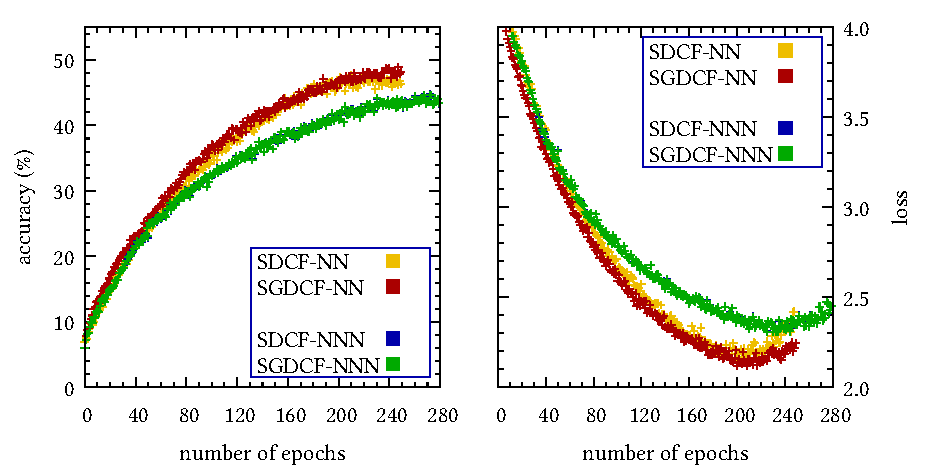
\includegraphics[width=1.1\textwidth]{./experiments/image-classification/comparison-token-mixers/graph-conv/graph-conv.pdf}}
    \caption{
        Comparison of the behavior of the traditional convolution based conformers (yellow and blue) to the graph based ones for image training data.
        The Blue and the green curve are completely identical (but calculated by optimizing different models), therefore blue is not visible.
        The reason, why the red and yellow curve are not also identical is due to different uses of the random number generator.
    }
    \label{fig:graph-convolution-works}
\end{figure}

The data clearly shows, that the implementations of SDCF-NNN and SGDCF-NNN behave exactly identical, even though they compute the path interactions with different operations, as they are mathematically identical.

It is natural to expect, that SDCF-NN and SGDCF-NN behave likewise, but slight differences in the data of theses two be observed.
This is because of the pseudo random number generator used in PyTorch.
The implementation of the graph-convolution (\emph{GraphMaskConvolution} in \cite{selfComputerScience} \filepath{/models/metaformer.py}) and the conventional-convolution (\emph{SymmDepthSepConv2d} in \cite{selfComputerScience} \filepath{/models/helpers/SymmConv2d.py}) query the random number generator a different number of times, because the graph implementation always allocates ($3 \cdot \mathrm{channels}$) weights and the conventional implementation only allocates ($2 \cdot \mathrm{channels}$) weights for nn interactions and ($3 \cdot \mathrm{channels}$) for nnn.
This causes the random number generator to drift apart and produces a propagating difference in the calculations \emph{only} for nn and not for nnn.

While this is a fixable flaw of the implementation, it clearly shows that the graph and non-graph implementations are behaving similar, even if the starting conditions are non-equivalent.
The comparison among the whole set of metaformers will emphasize how similar these two curves really are.

This proves, that convolutions can directly be translated into a graph context and motivates their function on non-tensor-like data structures.
